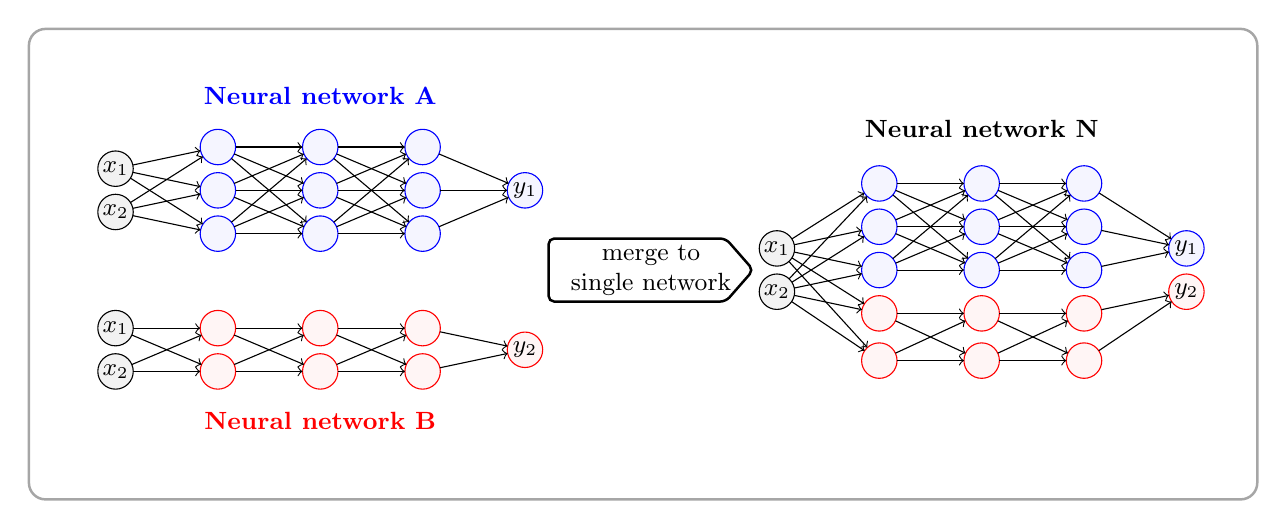
\begin{tikzpicture}[every node/.style={inner sep=0, outer sep=0, font=\small}]

  % parameters
  \def\circlesize{0.45cm}
  \def\colperc{4}
  \def\layersep{1.3} % horizontal step between layers
  \def\ysep{0.55} % vertical step between some neurons
  \def\inputOffset{0.5*\ysep} % half of \ysep, offset for input positions
  \def\yextra{0.05} % small extra used in network N bottom neuron

  % left x positions
  \pgfmathsetmacro{\xinputLeft}{-0.8} 
  \pgfmathsetmacro{\xhAone}{\xinputLeft+\layersep}
  \pgfmathsetmacro{\xhAtwo}{\xinputLeft+2*\layersep}
  \pgfmathsetmacro{\xhAthree}{\xinputLeft+3*\layersep}
  \pgfmathsetmacro{\xoutA}{\xinputLeft+4*\layersep}

  % right network x
  \pgfmathsetmacro{\rx}{7.6}
  \pgfmathsetmacro{\xhNOne}{\rx+\layersep}
  \pgfmathsetmacro{\xhNTwo}{\rx+2*\layersep}
  \pgfmathsetmacro{\xhNThree}{\rx+3*\layersep}
  \pgfmathsetmacro{\xoutN}{\rx+4*\layersep}

  % vertical centers
  \pgfmathsetmacro{\yCenterA}{2.0} % center for network A
  \pgfmathsetmacro{\yCenterB}{-0.025} % center for network B
  \pgfmathsetmacro{\yCenterN}{0.9875} % center for network N

  % N y positions
  \pgfmathsetmacro{\yNtop}{\yCenterN + 2*\ysep}
  \pgfmathsetmacro{\yNnext}{\yCenterN + 1*\ysep}
  \pgfmathsetmacro{\yNmid}{\yCenterN}
  \pgfmathsetmacro{\yNnextdown}{\yCenterN - 1*\ysep}
  \pgfmathsetmacro{\yNbottom}{\yCenterN - (2*\ysep + \yextra)}

  %---------------------------------
  % Neural network A (top-left)
  %---------------------------------

  % Input
  \node[draw, circle, minimum size=\circlesize, fill=gray!10]
    (n1-in1) at (\xinputLeft, {\yCenterA+\inputOffset}) {$x_{1}$};
  \node[draw, circle, minimum size=\circlesize, fill=gray!10]
    (n1-in2) at (\xinputLeft, {\yCenterA-\inputOffset}) {$x_{2}$};

  % Hidden 1
  \node[draw=blue, fill=blue!\colperc, circle, minimum size=\circlesize]
    (n1-h1-1) at (\xhAone, {\yCenterA+\ysep}) {};
  \node[draw=blue, fill=blue!\colperc, circle, minimum size=\circlesize]
    (n1-h1-2) at (\xhAone, {\yCenterA}) {};
  \node[draw=blue, fill=blue!\colperc, circle, minimum size=\circlesize]
    (n1-h1-3) at (\xhAone, {\yCenterA-\ysep}) {};

  % Hidden 2
  \node[draw=blue, fill=blue!\colperc, circle, minimum size=\circlesize]
    (n1-h2-1) at (\xhAtwo, {\yCenterA+\ysep}) {};
  \node[draw=blue, fill=blue!\colperc, circle, minimum size=\circlesize]
    (n1-h2-2) at (\xhAtwo, {\yCenterA}) {};
  \node[draw=blue, fill=blue!\colperc, circle, minimum size=\circlesize]
    (n1-h2-3) at (\xhAtwo, {\yCenterA-\ysep}) {};

  % Hidden 3
  \node[draw=blue, fill=blue!\colperc, circle, minimum size=\circlesize]
    (n1-h3-1) at (\xhAthree, {\yCenterA+\ysep}) {};
  \node[draw=blue, fill=blue!\colperc, circle, minimum size=\circlesize]
    (n1-h3-2) at (\xhAthree, {\yCenterA}) {};
  \node[draw=blue, fill=blue!\colperc, circle, minimum size=\circlesize]
    (n1-h3-3) at (\xhAthree, {\yCenterA-\ysep}) {};

  % Output
  \node[draw=blue, fill=blue!\colperc, circle, minimum size=\circlesize]
    (y_1_left) at (\xoutA, {\yCenterA}) {$y_{1}$};

  % Label
  \node[font=\small\bfseries, text=blue]
    at ({(\xhAtwo)}, {\yCenterA+1.2}) {Neural network A};


  % Connections A
  \foreach \i in {1,2} {
    \foreach \j in {1,2,3} {
      \draw[->] (n1-in\i) -- (n1-h1-\j);
    }
  }
  \foreach \i in {1,2,3} {
    \foreach \j in {1,2,3} {
      \draw[->] (n1-h1-\i) -- (n1-h2-\j);
      \draw[->] (n1-h2-\i) -- (n1-h3-\j);
    }
    \draw[->] (n1-h3-\i) -- (y_1_left);
  }


  %---------------------------------
  % Neural network B (bottom-left)
  %---------------------------------

  % Input
  \node[draw, circle, minimum size=\circlesize, fill=gray!10]
    (n2-in1) at (\xinputLeft, {\yCenterB+\inputOffset}) {$x_{1}$};
  \node[draw, circle, minimum size=\circlesize, fill=gray!10]
    (n2-in2) at (\xinputLeft, {\yCenterB-\inputOffset}) {$x_{2}$};

  % Hidden 1
  \node[draw=red, fill=red!\colperc, circle, minimum size=\circlesize]
    (n2-h1-1) at (\xhAone, {\yCenterB+\inputOffset}) {};
  \node[draw=red, fill=red!\colperc, circle, minimum size=\circlesize]
    (n2-h1-2) at (\xhAone, {\yCenterB-\inputOffset}) {};

  % Hidden 2
  \node[draw=red, fill=red!\colperc, circle, minimum size=\circlesize]
    (n2-h2-1) at (\xhAtwo, {\yCenterB+\inputOffset}) {};
  \node[draw=red, fill=red!\colperc, circle, minimum size=\circlesize]
    (n2-h2-2) at (\xhAtwo, {\yCenterB-\inputOffset}) {};

  % Hidden 3
  \node[draw=red, fill=red!\colperc, circle, minimum size=\circlesize]
    (n2-h3-1) at (\xhAthree, {\yCenterB+\inputOffset}) {};
  \node[draw=red, fill=red!\colperc, circle, minimum size=\circlesize]
    (n2-h3-2) at (\xhAthree, {\yCenterB-\inputOffset}) {};

  % Output
  \node[draw=red, fill=red!\colperc, circle, minimum size=\circlesize]
    (y_2_left) at (\xoutA, {\yCenterB}) {$y_{2}$};

  % Label
  \node[font=\small\bfseries, text=red]
    at ({(\xhAtwo)}, {\yCenterB-0.9}) {Neural network B};


  % connections B
  \foreach \i in {1,2} {
    \foreach \j in {1,2} {
      \draw[->] (n2-in\i) -- (n2-h1-\j);
      \draw[->] (n2-h1-\i) -- (n2-h2-\j);
      \draw[->] (n2-h2-\i) -- (n2-h3-\j);
    }
  }
  \foreach \i in {1,2} { 
    \draw[->] (n2-h3-\i) -- (y_2_left); }


  %---------------------------------
  % Neural network N (right)
  %---------------------------------

  % Input
  \node[draw, circle, minimum size=\circlesize, fill=gray!10]
    (n3-in1) at (\rx, {\yCenterN+\inputOffset}) {$x_{1}$};
  \node[draw, circle, minimum size=\circlesize, fill=gray!10]
    (n3-in2) at (\rx, {\yCenterN-\inputOffset}) {$x_{2}$};

  % Hidden 1 (5 neurons)
  \node[draw=blue, fill=blue!\colperc, circle, minimum size=\circlesize]
    (n3-h1-1) at (\xhNOne, {\yNtop}) {};
  \node[draw=blue, fill=blue!\colperc, circle, minimum size=\circlesize]
    (n3-h1-2) at (\xhNOne, {\yNnext}) {};
  \node[draw=blue, fill=blue!\colperc, circle, minimum size=\circlesize]
    (n3-h1-3) at (\xhNOne, {\yNmid}) {};
  \node[draw=red,  fill=red!\colperc,  circle, minimum size=\circlesize]
    (n3-h1-4) at (\xhNOne, {\yNnextdown}) {};
  \node[draw=red,  fill=red!\colperc,  circle, minimum size=\circlesize]
    (n3-h1-5) at (\xhNOne, {\yNbottom}) {};

  % Hidden 2
  \node[draw=blue, fill=blue!\colperc, circle, minimum size=\circlesize]
    (n3-h2-1) at (\xhNTwo, {\yNtop}) {};
  \node[draw=blue, fill=blue!\colperc, circle, minimum size=\circlesize]
    (n3-h2-2) at (\xhNTwo, {\yNnext}) {};
  \node[draw=blue, fill=blue!\colperc, circle, minimum size=\circlesize]
    (n3-h2-3) at (\xhNTwo, {\yNmid}) {};
  \node[draw=red,  fill=red!\colperc,  circle, minimum size=\circlesize]
    (n3-h2-4) at (\xhNTwo, {\yNnextdown}) {};
  \node[draw=red,  fill=red!\colperc,  circle, minimum size=\circlesize]
    (n3-h2-5) at (\xhNTwo, {\yNbottom}) {};

  % Hidden 3
  \node[draw=blue, fill=blue!\colperc, circle, minimum size=\circlesize]
    (n3-h3-1) at (\xhNThree, {\yNtop}) {};
  \node[draw=blue, fill=blue!\colperc, circle, minimum size=\circlesize]
    (n3-h3-2) at (\xhNThree, {\yNnext}) {};
  \node[draw=blue, fill=blue!\colperc, circle, minimum size=\circlesize]
    (n3-h3-3) at (\xhNThree, {\yNmid}) {};
  \node[draw=red,  fill=red!\colperc,  circle, minimum size=\circlesize]
    (n3-h3-4) at (\xhNThree, {\yNnextdown}) {};
  \node[draw=red,  fill=red!\colperc,  circle, minimum size=\circlesize]
    (n3-h3-5) at (\xhNThree, {\yNbottom}) {};

  % Output
  \node[draw=blue, fill=blue!\colperc, circle, minimum size=\circlesize]
    (y_right_top) at (\xoutN, {\yCenterN+\inputOffset}) {$y_{1}$};
  \node[draw=red,  fill=red!\colperc,  circle, minimum size=\circlesize]
    (y_right_bot) at (\xoutN, {\yCenterN-\inputOffset}) {$y_{2}$};

  % Label
  \node[font=\small\bfseries] at ({\xhNTwo}, {\yCenterN+1.788}) {Neural network N};


  % Connections N
  \foreach \i in {1,2} {
    \foreach \j in {1,...,5} {
      \draw[->] (n3-in\i) -- (n3-h1-\j);
    }
  }
  \foreach \from/\to in {1/2,2/3} {
    \foreach \i in {1,2,3} {
      \foreach \j in {1,2,3} { 
        \draw[->] (n3-h\from-\i) -- (n3-h\to-\j); }
    }
    \foreach \i in {4,5} {
      \foreach \j in {4,5} { 
        \draw[->] (n3-h\from-\i) -- (n3-h\to-\j); }
    }
  }
  \foreach \i in {1,2,3} { 
    \draw[->] (n3-h3-\i) -- (y_right_top); }
  \foreach \i in {4,5} { 
    \draw[->] (n3-h3-\i) -- (y_right_bot); }



  % Arrow (box)
  \path (4.7, 0.5875) coordinate (A)
        (6.95, 0.5875) coordinate (B)
        (7.3, 0.9875)  coordinate (C)
        (6.95, 1.3875) coordinate (D)
        (4.7, 1.3875)  coordinate (E);
  \draw[draw=black, fill=white, line width=0.9pt, rounded corners=2pt]
    (A) -- (B) -- (C) -- (D) -- (E) -- cycle;
  \node[align=center,font=\small] at (6.0, 0.9875) {merge to\\single network};


  % Border
  \draw[line width=0.9pt, gray!70, rounded corners=6pt]
    (-1.9, -1.925) rectangle (13.7, 4.05);

\end{tikzpicture}